\documentclass{ctexbeamer}

\usepackage{packages}
\usepackage{mathstyle}

\graphicspath{{./images/}}

\usetheme{Madrid}
\beamertemplatenavigationsymbolsempty
\setbeamertemplate{caption}[numbered]

\title[数据重上传量子分类器复现]{基于数据重上传的通用量子分类器复现}
\subtitle{理论分析与数值实验}
\author[崔正平, 张译夫, 张扬皓]{崔正平, 张译夫, 张扬皓}
\institute[]{课程大作业汇报}
\date{}

\begin{document}

\begin{frame}
    \titlepage
\end{frame}

\section{理论部分}

\begin{frame}{核心问题与基本思想}
    \framesubtitle{理论部分 · 崔正平}
    \begin{columns}[T]
        \begin{column}{0.46\textwidth}
            \textbf{核心问题}
            \begin{itemize}
                \setlength{\itemsep}{1.0ex}
                \item 如何把经典输入 $\bm{x}$ 编码进量子电路, 并通过测量输出类别?
                \item 如果只编码一次数据, 后续固定旋转对所有输入作用相同, 难以形成复杂决策边界.
                \item 我们希望在量子比特数很少时仍获得足够的非线性表达能力.
            \end{itemize}
        \end{column}
        \begin{column}{0.50\textwidth}
            \textbf{数据重上传思想}
            \begin{itemize}
                \setlength{\itemsep}{1.0ex}
                \item 在每一层重新读取同一个输入.
                \item 各层使用可训练的数据权重与旋转偏置.
                \item 多层旋转逐步形成输入依赖的量子态.
            \end{itemize}
            \[
                \ket{0}\xrightarrow{L_1}\cdots
                \xrightarrow{L_N}\ket{\psi(\bm{x})}
                \longrightarrow\widehat c .
            \]
        \end{column}
    \end{columns}
    \vspace{0.4em}
    \begin{center}
        \textcolor{blue}{用多次数据编码提高少量量子比特的分类表达能力.}
    \end{center}
    \vfill
    {\tiny Source: Pérez-Salinas et al., Quantum 4, 226 (2020).}
\end{frame}

\begin{frame}{理论基础: 量子态, Bloch 球与保真度}
    \framesubtitle{理论部分 · 崔正平}
    \begin{columns}[T]
        \begin{column}{0.48\textwidth}
            \textbf{量子态的 Bloch 表示}
            \[
                \rho=\frac12\left(I+\bm{r}\cdot\bm{\sigma}\right),
                \qquad r_i=\operatorname{tr}(\rho\sigma_i).
            \]
            \begin{itemize}
                \setlength{\itemsep}{0.9ex}
                \item $\bm{\sigma}=(\sigma_x,\sigma_y,\sigma_z)$ 是 Pauli 矩阵组.
                \item $\bm{r}$ 是 Bloch 向量; 纯态满足 $|\bm{r}|=1$, 混合态满足 $|\bm{r}|<1$.
            \end{itemize}
        \end{column}
        \begin{column}{0.48\textwidth}
            \textbf{分类的几何解释}
            \[
                F_c(\bm{x})
                =\operatorname{tr}\!\left[\rho_c\rho(\bm{x})\right]
                =\frac{1+\bm{s}_c\cdot\bm{r}(\bm{x})}{2}.
            \]
            \begin{itemize}
                \setlength{\itemsep}{0.9ex}
                \item 最大化 $F_c$ 就是让输出方向接近第 $c$ 类标签方向 $\bm{s}_c$.
                \item 二分类使用相反方向; 四分类使用正四面体顶点.
                \item 最终预测为 $\widehat c=\arg\max_c F_c(\bm{x})$.
            \end{itemize}
        \end{column}
    \end{columns}
\end{frame}

\begin{frame}{实际电路设计与训练流程}
    \framesubtitle{理论部分 · 崔正平}
    第 $i$ 层先将数据和可训练参数组成旋转角, 再施加单量子比特旋转:
    \[
        \bm{\phi}_i(\bm{x})=\bm{\theta}_i+\bm{w}_i\circ\bm{x},
        \qquad
        L_i(\bm{x})=U\!\left(\bm{\phi}_i(\bm{x})\right).
    \]
    \[
        \ket{0}
        \xrightarrow{U(\bm{\phi}_1)}
        \cdots
        \xrightarrow{U(\bm{\phi}_N)}
        \ket{\psi(\bm{x})}
        \xrightarrow{F_c(\bm{x})}
        \widehat c .
    \]
    \begin{enumerate}
        \setlength{\itemsep}{0.9ex}
        \item \textbf{编码:} $\bm{w}_i$ 缩放输入, $\bm{\theta}_i$ 提供可训练偏置.
        \item \textbf{演化:} 同一输入经过 $N$ 次重上传, 得到输出态 $\ket{\psi(\bm{x})}$.
        \item \textbf{测量:} 计算输出态与各类别标签态的保真度 $F_c(\bm{x})$.
        \item \textbf{更新:} 经典优化器根据训练损失更新 $\bm{\theta}_i$, $\bm{w}_i$ 及类别权重.
    \end{enumerate}
\end{frame}

\begin{frame}{表达能力与优化方法}
    \framesubtitle{理论部分 · 崔正平}
    \begin{columns}[T]
        \begin{column}{0.52\textwidth}
            \textbf{为什么能够产生非线性}
            \begin{itemize}
                \setlength{\itemsep}{0.9ex}
                \item 旋转轴之间通常不对易, 因而各层不能简单合并.
                \item 多层乘积产生交叉项及不同频率的三角函数组合.
                \item 增加重上传层通常提高表达能力, 但也会增加优化难度.
            \end{itemize}
        \end{column}
        \begin{column}{0.44\textwidth}
            \textbf{如何训练}
            \[
                \chi_f^2
                =\sum_\mu\left[1-F_{s_\mu}(\bm{x}_\mu)\right]^2.
            \]
            \[
                \min_{\bm{p}}\chi^2(\bm{p}),
                \qquad \ell_j\leq p_j\leq u_j.
            \]
            \begin{itemize}
                \setlength{\itemsep}{0.8ex}
                \item $\bm{p}$ 汇总旋转参数, 数据权重和类别权重.
                \item L-BFGS-B 用有限组历史向量近似逆 Hessian, 无需存储完整矩阵.
            \end{itemize}
        \end{column}
    \end{columns}
\end{frame}

\section{第一组实验}

\begin{frame}{实验 1--3 依次检验损失, 电路结构与剪枝}
    \framesubtitle{第一组实验 · 张扬皓}
    \begin{columns}[T]
        \begin{column}{0.46\textwidth}
            \textbf{统一任务与配置}
            \begin{itemize}
                \setlength{\itemsep}{0.9ex}
                \item 圆形二分类:
                \[
                    x_1^2+x_2^2<\frac{2}{\pi}.
                \]
                \item 训练/测试样本数: $200/4000$.
                \item 五个参数初始化随机种子.
                \item Python 状态向量模拟, L-BFGS-B 优化.
            \end{itemize}
        \end{column}
        \begin{column}{0.50\textwidth}
            \textbf{三个问题}
            \begin{enumerate}
                \setlength{\itemsep}{1.3ex}
                \item 重叠模损失与保真度损失是否等价?
                \item 减少层数, 增加量子比特或加入 CZ 能否保持性能?
                \item 删除一个完整的重上传层能否真正降低资源消耗?
            \end{enumerate}
        \end{column}
    \end{columns}
\end{frame}

\begin{frame}{实验 1--3: 改变目标或结构都会影响性能}
    \framesubtitle{第一组实验 · 张扬皓}
    \begin{itemize}
        \setlength{\itemsep}{1.2ex}
        \item \textbf{实验 1: 损失函数.} 相同初值下, 重叠模损失与保真度损失的平均准确率分别为 $0.88$ 和 $0.84$. 两者对应不同优化目标, 不能直接互换.
        \item \textbf{实验 2: 电路结构.} 1Q-L4 基准准确率为 $0.84$; 1Q-L2, 2Q-L2 无纠缠和 2Q-L2 CZ 分别为 $0.79$, $0.52$ 和 $0.60$, 均未保持基准性能.
        \item \textbf{实验 3: 层剪枝.} L4$\to$L3 后准确率由 $0.84$ 降至 $0.82$; 未优化线路深度由 $20$ 降至 $15$, 但优化编译后的深度仍为 $5$.
    \end{itemize}
    \vspace{0.5em}
    \begin{center}
        \textcolor{blue}{减少参数或增加量子比特, 都不会自动转化为精度与编译资源收益.}
    \end{center}
\end{frame}

\begin{frame}{实验 4: 大多数样本在 128 shots 后即可停止}
    \framesubtitle{第一组实验 · 张扬皓}
    \begin{columns}[T]
        \begin{column}{0.55\textwidth}
            \centering
            \begin{tikzpicture}
                \begin{axis}[
                    width=\linewidth,
                    height=0.58\textheight,
                    ybar,
                    bar width=9pt,
                    ymin=0,
                    ymax=100,
                    ylabel={停止比例/\%},
                    symbolic x coords={128,512,2048},
                    xtick=data,
                    xlabel={停止时累计 shots},
                    legend style={at={(0.98,0.98)},anchor=north east,font=\scriptsize,draw=none},
                    tick label style={font=\scriptsize},
                    label style={font=\scriptsize},
                    enlarge x limits=0.20
                ]
                    \addplot[fill=blue!65,draw=blue!80,nodes near coords={\pgfmathprintnumber[fixed,precision=1,fixed zerofill]{\pgfplotspointmeta}},every node near coord/.append style={font=\tiny,xshift=-3pt}] coordinates {(128,83.17) (512,8.85) (2048,7.98)};
                    \addlegendentry{L4 基准}
                    \addplot[fill=orange!75,draw=orange!90!black,nodes near coords={\pgfmathprintnumber[fixed,precision=1,fixed zerofill]{\pgfplotspointmeta}},every node near coord/.append style={font=\tiny,xshift=3pt}] coordinates {(128,81.98) (512,9.39) (2048,8.63)};
                    \addlegendentry{L4--L3 剪枝}
                \end{axis}
            \end{tikzpicture}
        \end{column}
        \begin{column}{0.41\textwidth}
            \textbf{准确率与平均 shots}
            \vspace{0.4em}
            \begin{table}
                \centering
                \small
                \renewcommand{\arraystretch}{1.25}
                \begin{tabular}{lcc}
                    \toprule
                    模型 & 准确率 & shots \\
                    \midrule
                    L4 & $0.82\pm0.03$ & 315.2 \\
                    剪枝 L3 & $0.81\pm0.02$ & 329.8 \\
                    \bottomrule
                \end{tabular}
            \end{table}
            \begin{itemize}
                \setlength{\itemsep}{0.9ex}
                \item 与固定 2048 shots 的准确率差小于 $0.005$.
                \item 平均测量成本减少约 $84\%$.
                \item 结果来自理想有限测量模拟.
            \end{itemize}
        \end{column}
    \end{columns}
\end{frame}

\section{第二组实验}

\begin{frame}{第二组实验在五类任务上系统扫描配置}
    \framesubtitle{第二组实验 · 张译夫}
    \begin{columns}[T]
        \begin{column}{0.48\textwidth}
            \textbf{五类分类任务}
            \begin{itemize}
                \setlength{\itemsep}{0.7ex}
                \item 非凸边界
                \item 二分类圆环
                \item 三维球
                \item 四分类方块
                \item 四分类波浪线
            \end{itemize}
            \textbf{配置网格}
            \begin{itemize}
                \setlength{\itemsep}{0.7ex}
                \item 层数: $1,2,3,4,5,6,8,10$.
                \item 非加权/加权保真度损失.
                \item $1/2/4$ 量子比特, 有/无 CZ.
                \item 合计 $5\times61=305$ 次训练.
            \end{itemize}
        \end{column}
        \begin{column}{0.48\textwidth}
            \centering
            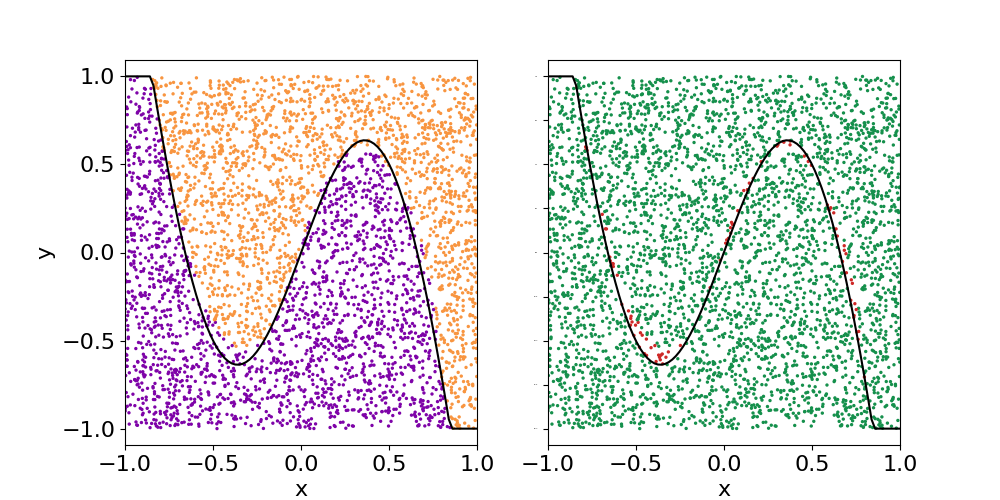
\includegraphics[width=\textwidth]{non_convex.png}

            {\scriptsize 非凸边界示例: 左侧为数据标签, 右侧为模型预测区域.}
        \end{column}
    \end{columns}
\end{frame}

\begin{frame}{层数带来最稳定增益, 其他因素依赖具体任务}
    \framesubtitle{第二组实验 · 张译夫}
    \centering
    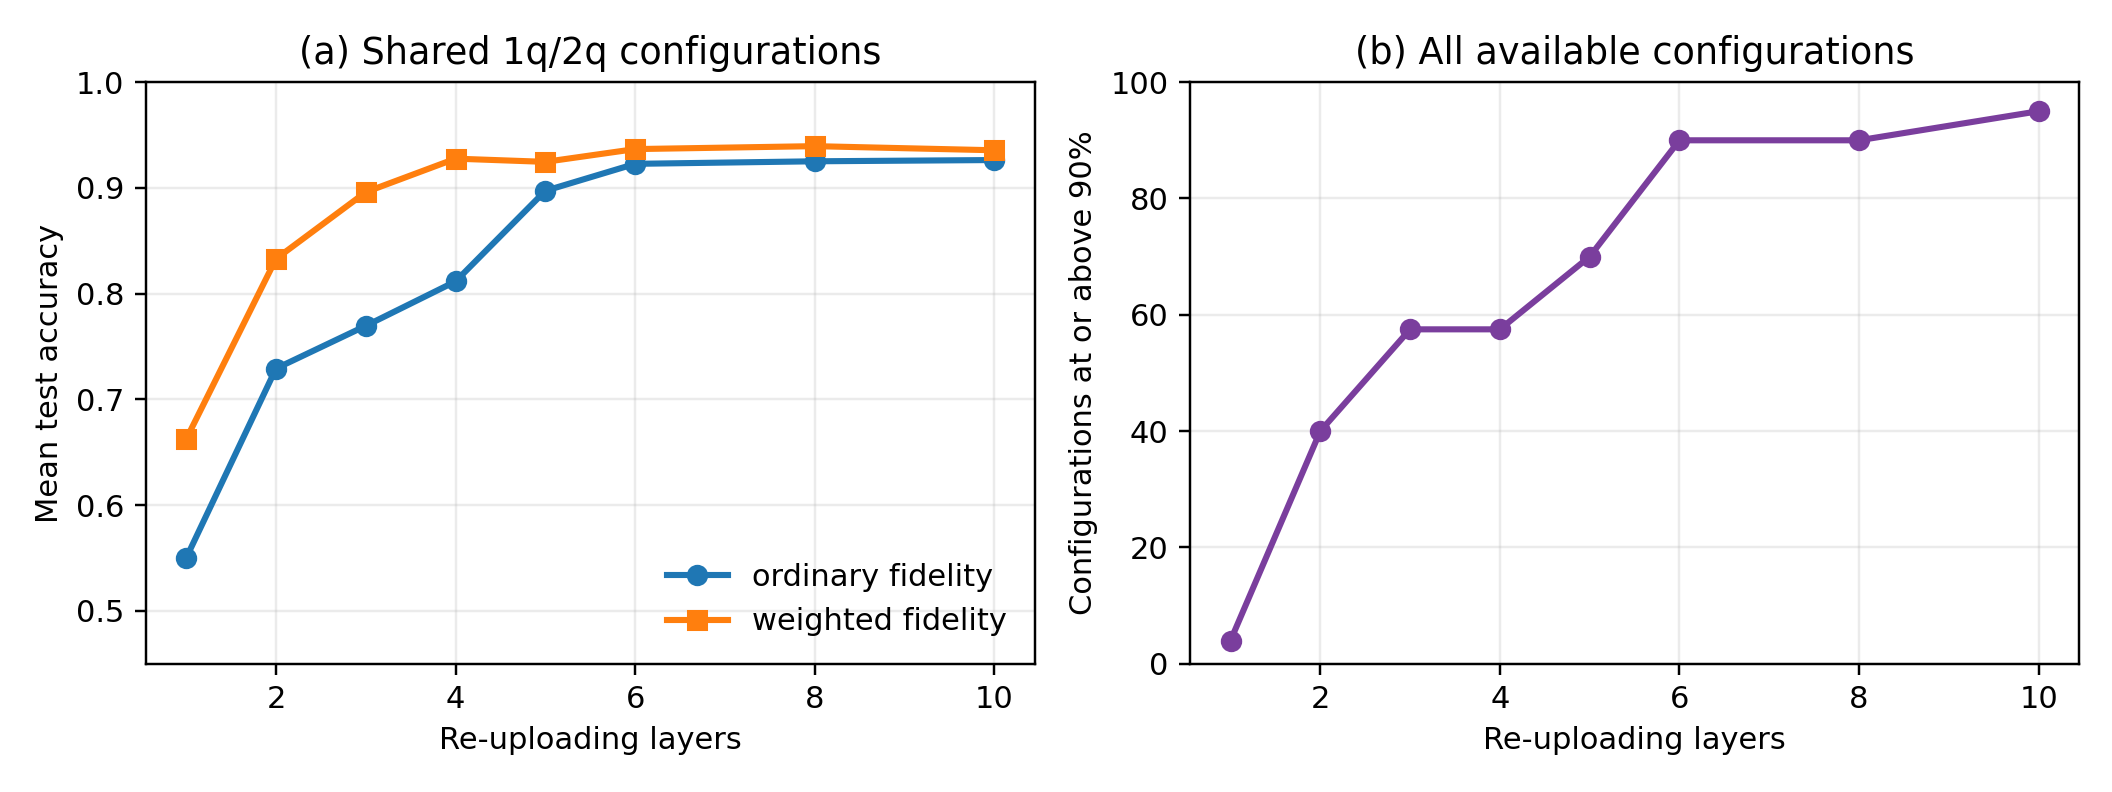
\includegraphics[width=0.91\textwidth]{layer_trends.png}
    \vspace{-0.2em}
    \begin{itemize}
        \setlength{\itemsep}{0.55ex}
        \item 平均性能主要在前 $5$--$6$ 层提升, 随后进入平台区.
        \item 在 $115$ 对共享配置上, 加权损失平均提高 $6.34$ 个百分点, 但并非每类任务都占优.
        \item 在 $105$ 对纠缠比较中, CZ 的平均增益仅为 $0.53$ 个百分点且正负并存.
    \end{itemize}
\end{frame}

\begin{frame}{一个典型案例: CZ 将圆环准确率提高到 96\%}
    \framesubtitle{第二组实验 · 张译夫}
    \begin{columns}[T]
        \begin{column}{0.48\textwidth}
            \centering
            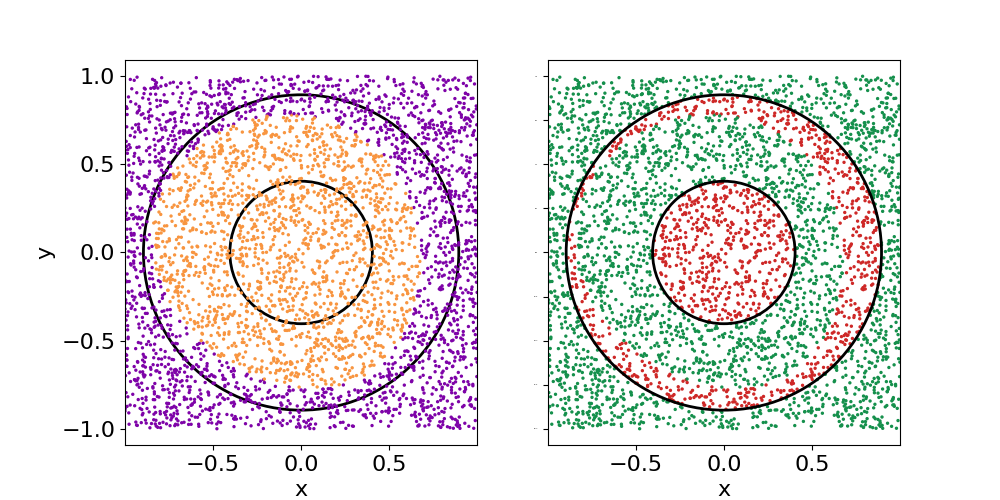
\includegraphics[width=\textwidth]{crown_4q_l2_separable.png}

            {\small 无 CZ: 70.45\%}
        \end{column}
        \begin{column}{0.48\textwidth}
            \centering
            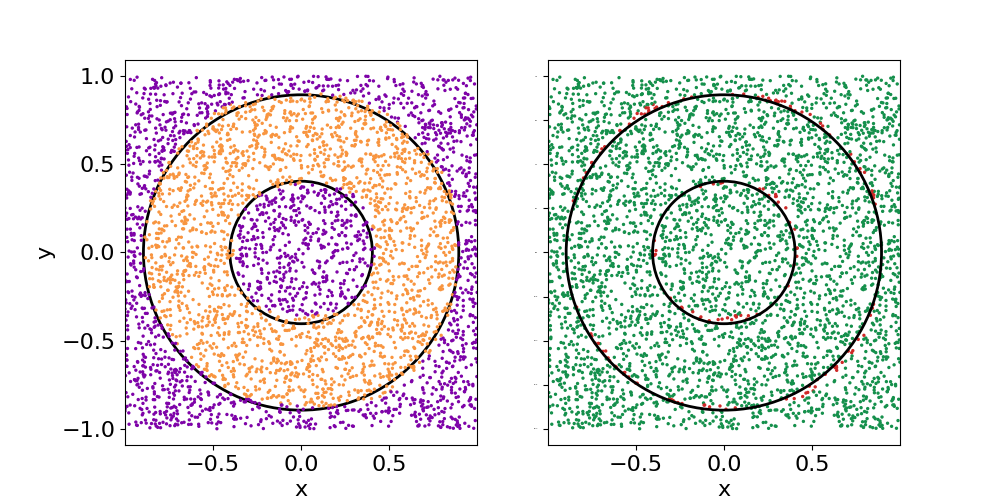
\includegraphics[width=\textwidth]{crown_4q_l2_entangled.png}

            {\small 加入 CZ: 96.00\%}
        \end{column}
    \end{columns}
    \vspace{0.5em}
    \begin{itemize}
        \setlength{\itemsep}{0.7ex}
        \item 两者均为 4 量子比特, 2 层, 加权保真度模型, 只改变是否加入纠缠门.
        \item 这是纠缠收益最大的实例; 在全部 105 对比较中, CZ 的平均增益仅为 $0.53$ 个百分点, 因而不能推广为普遍结论.
    \end{itemize}
\end{frame}

\begin{frame}{五类任务的最佳准确率均超过 93\%}
    \framesubtitle{第二组实验 · 张译夫}
    \begin{table}
        \centering
        \small
        \renewcommand{\arraystretch}{1.25}
        \begin{tabular}{lccccc}
            \toprule
            任务 & 最高准确率 & 损失 & 量子比特 & CZ & 层数 \\
            \midrule
            非凸边界 & 97.75\% & $\chi_{wf}^2$ & 2 & 无 & 8 \\
            二分类圆环 & 97.25\% & $\chi_{wf}^2$ & 2 & 无 & 5 \\
            三维球 & 96.17\% & $\chi_{wf}^2$ & 4 & 有 & 2 \\
            四分类方块 & 98.58\% & $\chi_f^2$ & 2 & 有 & 5 \\
            四分类波浪线 & 93.90\% & $\chi_{wf}^2$ & 4 & 有 & 8 \\
            \bottomrule
        \end{tabular}
    \end{table}
    \begin{itemize}
        \setlength{\itemsep}{0.7ex}
        \item 最优电路横跨 $2/4$ 量子比特, $2$--$8$ 层及有/无 CZ, 不存在统一最优结构.
        \item 上表是从 $305$ 个配置中按固定测试集准确率选出的描述性结果, 仍需验证集选择和多随机种子复核.
    \end{itemize}
\end{frame}

\begin{frame}{结论: 数据重上传有效, 资源收益仍需任务化验证}
    \framesubtitle{总结 · 张译夫}
    \begin{itemize}
        \setlength{\itemsep}{1.1ex}
        \item 多次输入编码与非对易旋转产生丰富的三角函数组合, 使少量量子比特能够表示复杂决策边界.
        \item 重上传层数是最稳定的容量来源; 加权保真度和纠缠结构的收益具有明显任务依赖性.
        \item 简单删层或增加量子比特不会自动带来更好的精度或更浅的编译电路; 
        \item 当前结果来自理想状态向量模拟, 随机种子数量有限, 尚未包含设备噪声, 真机实验和统一经典基线.
    \end{itemize}
\end{frame}

\begin{frame}
    \centering
    \Huge \textcolor{structure}{谢谢!}
\end{frame}

\end{document}
